%
% Chapter 2
%
\chapter{Background}\label{chap:background}

% Do an introduction to the chapter

\section{Introduction to the Problem}\label{sec:introduction-to-the-problem}
\paragraph{}

In today's fast paced world, the authenticity and accessibility of academic certificates play a crucial role in ensuring trust and credibility in various
domains, ranging from education to employment and beyond.
The current and traditional \textit{paper-based} system of issuing and verifying academic certificates is not only time consuming but also prone to a lot of fraud and manipulation.
The rampant proliferation of counterfeit certificates, inefficient verification processes and the risk of loss or damage highlight the need for a more reliable, robust and secure academic
certificate registry system.

The current system of academic certificate registry is plagued by numerous challenges. Firstly, the reliance and trust on paper-based certificates is a major issue
making them susceptible to forgery and tampering undermining the cridibility and integrity of academic qualifications. Secondly, the manual verification process is
time-consuming and prone to errors, leading to delays in credential validation, possible fraudulent activities and also potential loss of revenue for institutions due to
errors in the manual release. Thirdly, the centralized nature of certificate issuance by educational intituitions exacerbates the difficulty
of maintaining a unified and updated registry, hampering efficient verification mechanisms.

\section{Alternative Approaches}\label{sec:alternative-approaches}
\paragraph{}

Several attemps have been made to address the imperfections of the traditional academic certificate registry system.
One such solution is the implementation of \textit{centralized databases}~\cite{OLSON200971} managed by government or regulatory authorities, where educational institutions are required to
submit digital copies of certificates for verification purposes. Additionally this approach aims to centralize certificate records and simplify the verification process. However it still faces challenges
such as the risk and concerns of data privacy and security, interoperability issues between different databases and the need of a trusted third party to manage the database.
This centralized mechanism of keeping record is also devoted to have a single point of failure.
% missing examples of centralized databases

Another solution that is gaining traction is the adoption of \textit{blockchain technology} for academic certificate registry. Blockchain offers a decentralized, secure and tamper-proof ledger where certificates can be stored and verified.
The use of blockchain technology ensures that certificates are immutable, transparent and accessible to all stakeholders. Moreover, this technology enables the instant verification trough cryptographic methods,
eliminating the need for a central authority to manage the registry, thereby reducing the risk of fraud and manipulation.
This approach eliminates the need for a central authority to manage the registry, thereby reducing the risk of fraud and manipulation.

In contrast to the traditional centralized databased system, in our opinion, blockchain emerges as a disruptive force capable of revolutionizing academic certificate registry systems
by providing in a decentralized and secure manner, an immutable and tamper-proof ledger where certificates will be stored and verified.
The decision to embrace blockchain technology as the foundation of our solution is based on what we sad above as well as the fact that blockchain technology is a key enabler of the \textit{Web3} vision,
which aims to create decentralized applications (\textit{dApps}) that are secure, transparent and trustless where users have full control over their data and digital assets without having a \textbf{single point of failure}.
% missing examples of blockchain technology

\pagebreak % temporary solution to avoid the section title to be alone in the previous page

% tempo de duração de uma transação
\section{Distributed System}\label{sec:distributed-systems}
\paragraph{}

As we transition to a blockchain-based solution for our problem it is crucial to understand the foundational concepts that make this technology both revolutionary and reliable.
Central to blockchain's efficacy is the principle of \textit{distributed consensus}, which ensures the integrity, security and transparency of the ledger.
This next sections explore into the mechanics of distributed consensus, the broader vision of \textit{Web3} and other key concepts integral to understanding how blockchain can trasnform
academic certificate registry systems.

\subsection*{Blockchain Technology}\label{subsec:blockchain}
\paragraph{}

% Some history of blockchain 
Blockchain is a technology behind the cryptocurrency Bitcoin initially described by Satoshi Nakamoto in a 2008 white paper titled `Bitcoin: A Peer-to-Peer Electronic Cash System'~\cite{nakamoto2008bitcoin}.
Although the term blockchain gained popularity in that year, with the introduction of Bitcoin cryptocurrency by Nakamoto, its underlying concepts have been used since the 1980s.
Later in 2004, Harold Thomas Finney II (Hal Finney) introduced the Reusable Proof of Work (\textit{RPOW}) system~\cite{RPOW}. The RPOW system was a digital
currency system that used a \textit{proof-of-work} limit the amount of work done by the server and to limit the amount of work done by the client.
The RPOW system was the first system to use a blockchain-like structure to store and verify transactions. After sometime, in 2009 the first bitcoin transaction was made by Nakamoto
to his friend Hal Finney~\cite{peterson2014hal} where was tranfered 10 BTC (bitcoin). This marked the beginning of the blockchain technology era.
In 2013, Vitalik Buterin proposed the concept of \textit{smart contracts} in his white paper `Ethereum: The Ultimate Smart Contract and Decentralized Application Platform'~\cite{buterin2013ethereum}. Uppon this publication,
\textit{Ethereum} has launched his own blockchain in 2015.~\cite{reiff2020bitcoin}.

All of the above information is to show how blockchain has evolved over the past few years and is presented in~\cite{TRIPATHI2023100344}. % it is really necessary to have this information?

\subsubsection*{What is Blockchain?}\label{subsubsec:what-is-the-blockchain}
\paragraph{}

A blockchain is a time-ordered set of blocks where each block is cryptographically linked to the previous one forming a chain. All blocks are stored in a decentralized and distributed ledger and become
thrustworthy digital records whar are unmodifiable in practice but very easy to verify. Like mencioned in the previous section~\ref{sec:alternative-approaches} there is no centralized or hierarchical structure in the blockchain network
and the information is shared by a network of \textit{peers}.

\begin{figure}[h]\label{fig:blockchain}
    \begin{center}
        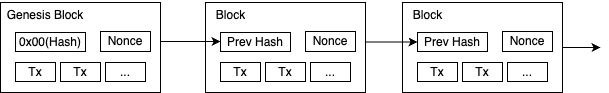
\includegraphics[width=0.8\textwidth]{assets/blockchain.png}
        \caption{Blockchain structure adapted from~\cite{nakamoto2008bitcoin}}
    \end{center}
\end{figure}

Each block contains a reliable register of one or more actually executed transactions that are created and exchanged by the network participants (peers) which eventually must modify
its state. To add new information to the chain, a \textbf{consensus} about its truthfulness must be reached among the peers in the network.

The content of each transaction that is stored in a single block depends on the specific type of blockchain and its prupose. In our case and very succinctly, the transaction has an `item' that contains information about
the academic certificate; we will discuss this in more detail in the next chapters. Other example used for the time being is the Bitcoin, where the main information registered are exchanges of
bitcoins between accounts.

Other important aspect of a chain node and the major reason for its security is the \textbf{hash}. The hash is a mathematical function that takes an input (or `message') and returns a fixed-size string of bytes.
This function is used to verify whether or not the data contained in the block has been tampered with. It is created when a new block is added or updated onto the chain.
In the blockchain, the hash of a block contains the information of the previous block's hash and any minimal change in the block's content will result in a completely different hash.
This is the reason why the blockchain is considered tamper-proof and secure.

Some blockchains support the use of \textit{Smart Contracts}~\cite{kaur2023introduction} which are a modern version of the tradition paper-based agreements mencioned before.
These Smart Contracts are a critical component of several applications and platforms using a distributed ledger technology that we will be using in out solution and for better understading we will explain with
more detail in the next sections.

There are three main types of blockchain~\cite{paul2021blockchain}:

\begin{itemize}
    \item {Public}: is called public if each participants can read and use it to carry out transactions but also
          if everyone can participate in the process of creating the \textbf{consensus} which can be \textit{Proof-of-Work} or \textit{Proof-of-Stake}.
          In this type of blockchain there is no central authority nor a trusted third party to control the network.
          Examples of this type of blockchain are \textbf{Bitcoin}~\cite{nakamoto2008bitcoin} and \textbf{Ethereum}~\cite{tual2015ethereum}. The main advantages of this type of blockchain are:
          \begin{itemize}
              \item High security and privacy,
              \item Open and Flexible Environment,
              \item No regulations,
              \item Full Transparency and Systems,
              \item Distributed, etc.
          \end{itemize}

    \item {Private}: these are restricted and not open, such kind of blockchain also haas features of access. This type of blockchains works mostly on closed systems and networks and are usually
          useful in organizations and companies which only selected members can join and access the data. Private blockchains have running only authorized nodes and that means that no one from the outside
          of the private network is able to access the information and data exchanged between two nodes. In this type there is no mining, no proof of work, and no remuneration~\cite{guegan:halshs-01524440}. 
          Examples of this type of blockchain are \textbf{Hyperledger Fabric}~\cite{hyperLedger} and \textbf{R3 Corda}~\cite{r3Corda}.
          The main advantages of this type of blockchain are:
          \begin{itemize}
              \item Full of privacy,
              \item High Efficiency,
              \item Faster Transaction,
              \item Better Scability,
          \end{itemize}
    \item {Consortium~\cite{KASI20221}}: a combination of both public and private blockchains. As in a private blockchain, participants may join the network only by invitation and must be approved by the network owner, however,
          there is not a single organization that has control over the network. Instead, the control is distributed among a group of participants.
          \begin{itemize}
              \item High Security,
              \item High Scalability,
              \item High Efficiency,
              \item High Privacy,
              \item High Flexibility,
          \end{itemize}

\end{itemize}

\subsection*{Distributed Consensus Mechanisms}\label{subsec:distributed-consensus-mechanisms}
\paragraph{}

Distributed consensus feature allows a blockchain-based system


\section{Differente Approaches to Blockchain}\label{sec:different-approaches-to-blockchain}
\paragraph{}




